% !TEX root = ./Vorlesungsmitschrift AGLA 2.tex  
\lecture{Fr 15.05. 10:15}{}
Resultate der affinen Hauptachsentransformation im \( \reals^2 \): \( m=\rang A \), \( m'=\rang A' \).
\begin{eigenschaftenenumerate}
  \item \( m=m' \):
  \begin{proofdescription}
    \item[\( m=m'=0 \):] \( Q \) gegeben durch \( 0=0 \) \tto Ebene \( \reals^2 \).
    \item[\( m=m'=1 \)] \( x_1^2=0 \) \tto \enquote{doppelte} Gerade. 
    \begin{figure}[H]
      \centering
      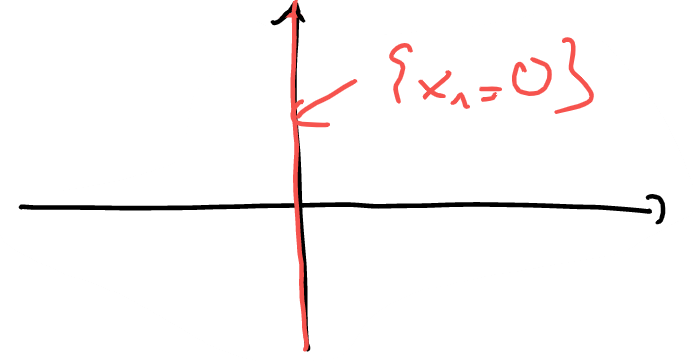
\includegraphics[width=0.5\linewidth]{figures/doppelte_gerade}
      \label{fig:doppelte_gerade}
    \end{figure}
    \item[\( m=m'=2 \)] \( x_1^2+x_2^2=0 \) \tto Punkt.
    \begin{figure}[H]
      \centering
      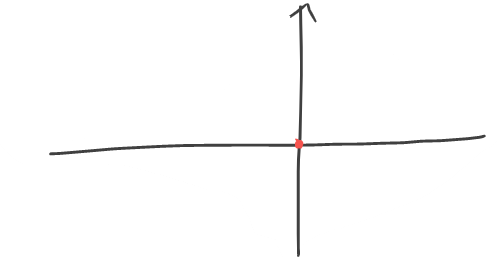
\includegraphics[width=0.5\linewidth]{figures/punkt_quadrik}
      \label{fig:punkt_quadrik}
    \end{figure}
    \item[\( \equalto{(x_1+x_2)(x_1-x_2)}{x_1^2-x_2^2}=0 \)] \tto 2 Geraden.
    \begin{figure}[H]
      \centering
      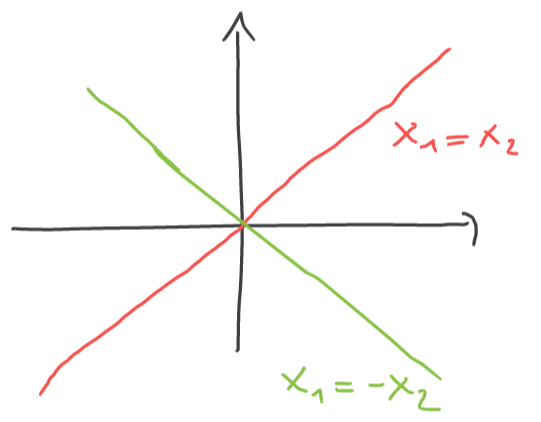
\includegraphics[width=0.5\linewidth]{figures/zwei_geraden_quadrik}
      \label{fig:zwei_geraden_quadrik}
    \end{figure}
  \end{proofdescription}
  \item \( m'=m+1 \).
  \begin{proofdescription}
    \item[\( m=0 \)] \tto \( 0=1 \)  \tto leere Menge.
    \item[\( m=1 \)] \begin{proofdescription}
      \item[\( x_1^2=1 \)]  \tto 2 parallele Geraden
      \begin{figure}[H]
        \centering
        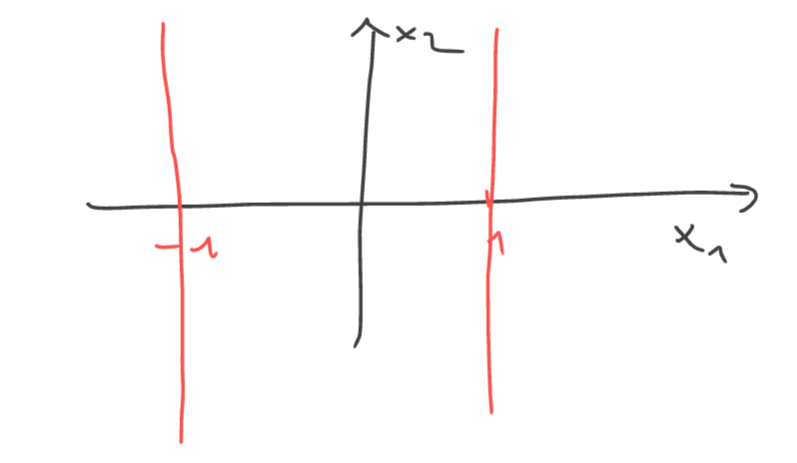
\includegraphics[width=0.5\linewidth]{figures/parallele_geraden_quadrik}
        \label{fig:parallele_geraden_quadrik}
      \end{figure}
      \item[\( -x_1^2=1 \)] \tto leere Menge.
    \end{proofdescription}
    \item[\( m=2 \)] \begin{proofdescription}
      \item[\( -x_1^2-x_2^2=1 \)] \tto \( \emptyset \).
      \item[\( x_1^2-x_2^2=1 \)] \tto Hyperbel. 
      \begin{figure}[H]
        \centering
        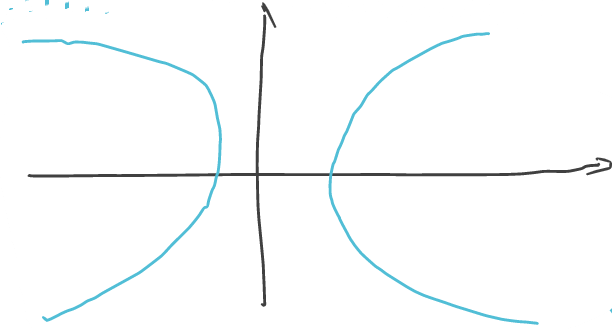
\includegraphics[width=0.5\linewidth]{figures/hyperbel_quadrik}
        \label{fig:hyperbel_quadrik}
      \end{figure}
      \item[\( x_1^2+x_2^2=1 \)] \tto Kreis.
      \begin{figure}[H]
        \centering
        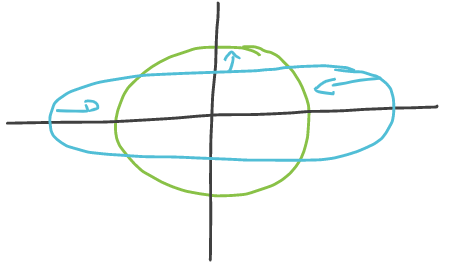
\includegraphics[width=0.5\linewidth]{figures/ellipse_kreis_quadrik}
        \label{fig:ellipse_kreis_quadrik }
      \end{figure}
    \end{proofdescription}
    \item \( m'=m+2 \). \begin{proofdescription}
      \item[\( m=0 \)] \begin{proofdescription}
        \item[\( 2x_1=0 \)] \tto Gerade.
      \end{proofdescription}
      \item[\( m=1 \)] \begin{proofdescription}
        \item[\( x_1^2+2x_2=0 \)] \tto Parabel.
        \begin{figure}[H]
          \centering
          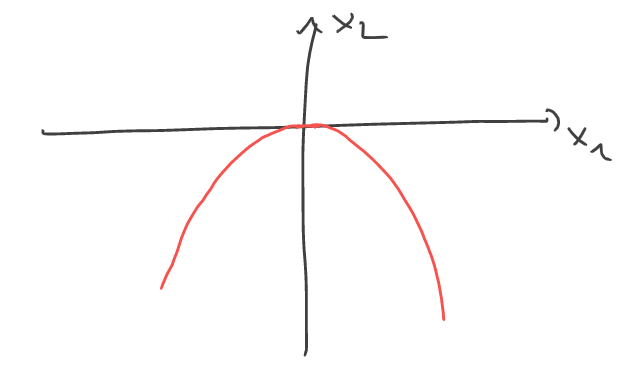
\includegraphics[width=0.5\linewidth]{figures/parabel_quadrik}
          \label{fig:parabel_quadrik}
        \end{figure}
      \end{proofdescription}
    \end{proofdescription}
  \end{proofdescription}
\end{eigenschaftenenumerate}
\begin{bemerkung*}
  Verschiedene dieser quadratischen Formen können als \emph{Menge} die gleiche Quadrik \( Q\subseteq \reals^2 \) beschreiben.
\end{bemerkung*}
\begin{beispiel*}
  \begin{equation*}
    \Set{(x_1,x_2)\in \reals^2|x_1^2=0}=\Set{(x_1,x_2)\subset \reals^2| 2x_1=0}.
  \end{equation*}
\end{beispiel*}
\begin{definition*}
  Wir nennen zwei Quadriken \( Q_1,Q_2\subseteq \reals^n \) \emph{geometrisch äquivalent} wenn es eine Affinität \( f\maps \reals^n\to \reals^n \) gibt mit \( f(Q_1)=Q_2 \).
\end{definition*}
\begin{frage*}
  Klassifikation aller Quadriken über \( \reals \) bis auf geometrische Äquivalenz?
\end{frage*}
Für eine Matrix \( B\in \matrices{n}{n}{\reals} \) sei \( \signature{B}=\anzahl-{} \) positive Eigenwerte von \( B \) \( -\anzahl-{} \) negative Eingenwerte von \( B \) die Signatur von \( B \).
\begin{satz}[Geometischer Klassifikationssatz (ohne Beweis)]
  Seien \( Q_1,Q_2\subset \reals^n \) nichtleere Quadriken, die beschrieben werden durch erweiterte Matrizen \( A_1',,A_2' \) mit rein quadratischen Anteilen \( A_1,A_2 \). Seien \( Q_1,Q_2 \) nicht gleich an Hyperebenen.

  Dann sind \( Q_1 \) und \( Q_2 \) \emph{geometrisch äquivalent} \gdw gilt
\begin{align*}
  \rang-{A_1}&=\rang-{A_2},\\
  \rang-{A_1'}&=\rang-{A_2'},\\
  \abs*{\signature-{A_1}}&=\abs*{\signature-{A_2}}\text{ und}\\
  \abs*{\signature-{A_1'}}&=\abs*{\signature-{A_2'}}.
\end{align*}
\end{satz}
\begin{folgerung}
  Sei \( Q\subset \reals^n \) eine nichtleere Quadrik. Dann ist \( Q \) geometrisch äquivalent zu genau einer der folgenden Quadriken.
  \begin{eigenschaftenenumerate}
    \item \label{quadriken_gleich_null_nur_quadrate}\( x_1^2+\dotsb+x_k^2-x_{k+1}^2-\dotsb-x_m^2=0 \), \( 0\leq k\leq m \), \( 2k-m\geq 0 \).
    \item \label{quadriken_gleich_eins}\( x_1^2+\dotsb+x_k^2-x_{k+1}^2-\dotsb-x_n^2=1 \), \( 1\leq k\leq m \).
    \item \label{qadriken_gleich_null_plus_ein_linearer}\( x_1^2+\dotsb+x_k^2-x_{k+1}-\dotsb-x_m^2+2x_{m+1}=0 \), \( 1\leq k\leq m \) und \( 2k-m\geq 0 \).
  \end{eigenschaftenenumerate}
\end{folgerung}
\begin{beispiele*}[Quadriken im \( \reals^3 \)]
  \begin{description}
    \item[Typ \ref{quadriken_gleich_null_nur_quadrate}] \( x_1^2+x_2^2-x_3^2=0 \)
    \begin{figure}[H]
      \centering
      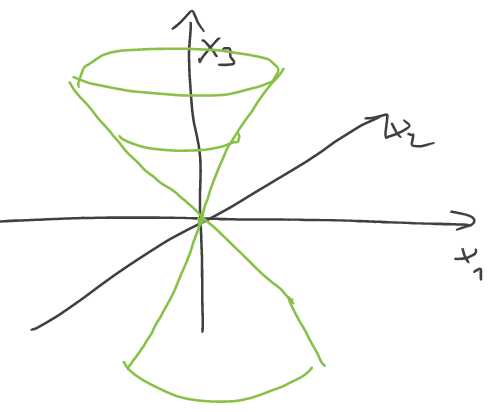
\includegraphics[width=0.5\linewidth]{figures/quadriken_beispiel_kegel}
      \caption*{Kegel}
      \label{fig:quadriken_beispiel_kegel}
    \end{figure}
    \item[Typ \ref{quadriken_gleich_eins}] \begin{itemize}
      \item \( x_1^2+x_2^2=1 \).
      \begin{figure}[H]
        \centering
        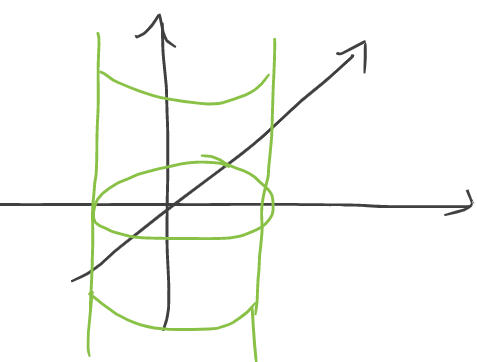
\includegraphics[width=0.5\linewidth]{figures/quadriken_beispiel_kreiszylinder}
        \caption*{Kreiszylinder}
        \label{fig:quadriken_beispiel_kreiszylinder}
      \end{figure}
      \item \( x_1^2+x_2^2+x_3^2=1 \).
      \begin{figure}[H]
        \centering
        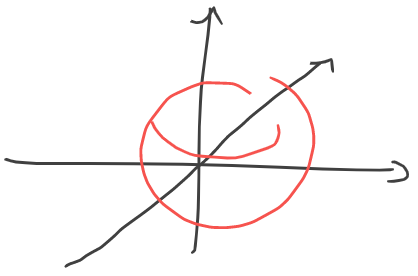
\includegraphics[width=0.5\linewidth]{figures/quadriken_beispiel_kugel}
        \caption*{Kugel}
        \label{fig:quadriken_beispiel_kugel}
      \end{figure}
      \item \( x_1^2-x_2^2+x_3^2=1 \).
      \begin{figure}[H]
        \centering
        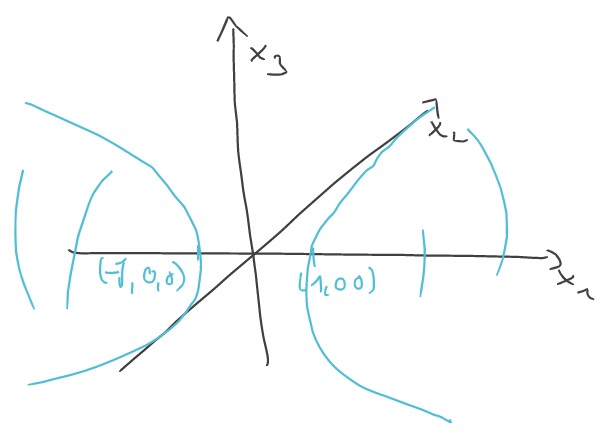
\includegraphics[width=0.5\linewidth]{figures/quadriken_beispiel_zweischaliges_hyperboloid}
        \caption*{Zweischaliges Hyperboloid}
        \label{fig:quadriken_beispiel_zweischaliges_hyperboloid}
      \end{figure}
      \item \( x_1^2+x_2^2-x_3^2=1 \)
      \begin{figure}[H]
        \centering
        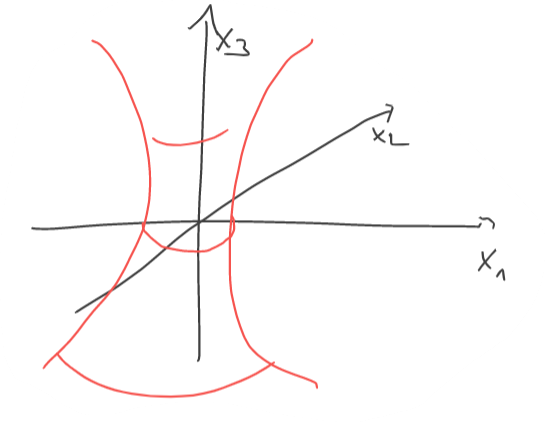
\includegraphics[width=0.5\linewidth]{figures/quadriken_beispiel_einschaliges_hyperboloid}
        \caption*{Einschaliges Hyperboloid}
        \label{fig:quadriken_beispiel_einschaliges_hyperboloid}
      \end{figure}
    \end{itemize}
    \item[Typ \ref{qadriken_gleich_null_plus_ein_linearer}] \( x_1^2+x_2^2+2x_3=0 \).
    \begin{figure}[H]
      \centering
      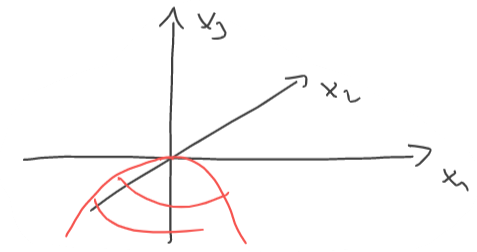
\includegraphics[width=0.5\linewidth]{figures/quadriken_beispiel_elliptisches_paraboloid}
      \caption*{Elliptisches Paraboloid}
      \label{fig:quadriken_beispiel_elliptisches_paraboloid}
    \end{figure}
  \end{description}
\end{beispiele*}
\file{Euklidische affine Räume}
\section{Euklidische affine Räume}
In einem allgemeinen affinen Raum \( X \) haben wir den Begriff von Gerade und parallelen Geraden (Sind \( L,L'\subset X \) Geraden, dann sagen wir, dass \( L \) und \( L' \) parallel sind, falls \( T(L)=T(L') \)).
\begin{figure}[H]
  \centering
  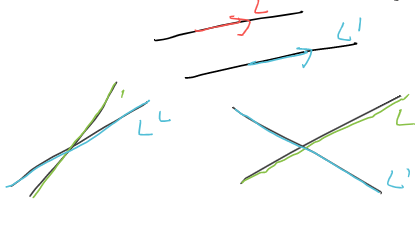
\includegraphics[width=0.5\linewidth]{figures/affine_geraden_lagebeziehungen}
  \label{fig:affine_geraden_lagebeziehungen}
\end{figure}
\begin{frage*}
  Können wir auch \enquote{Winkel} messen zischen zwei sich schneidenden Geraden?
\end{frage*}
\begin{erinnerung*}
  Sei \( V \) ein \( \reals \)-Vektorraum. Ein Skalarprodukt auf \( V \) ist eine \emph{positiv-definite symmetrische Bilinearform}
  \begin{equation*}
    S\maps V\times V\to \reals.
  \end{equation*}
\end{erinnerung*}
\begin{definition*}
  Ein euklidischer affiner Raum ist ein reeller affiner Raum \( (X,T(X),\tau) \) zusammen mit einem Skalarprodukt
  \begin{equation*}
    \scalarproduct{\cdot}{\cdot}\maps T(X)\times T(X)\to \reals
  \end{equation*}
  auf dem Translationsvektorraum \( T(X) \).
\end{definition*}
\begin{beispiel}
  Der \( \reals^n \) als reeller affiner Raum mit dem Standard-Skalarprodukt
  \begin{equation*}
    \begin{split}
      \scalarproduct{\cdot}{\cdot}\maps \underrelate{\vertrelation{\simeq}}{\reals^n}{T(X)}\times \underrelate{\vertrelation{\simeq}}{\reals^n}{T(X)}&\to \reals\\
      (x_1,\dotsc,x_n)\times (y_1,\dotsc,y_n)&\mapsto \sum_{i=1}^{n}x_i y_i.
    \end{split}
  \end{equation*}
\end{beispiel}
\begin{beispiel}
  Die Lösungsmenge \( L \) im \( \reals^n \) eines Systems von linearen Gleichungen \( Ax=b \), \( A\in \matrices{m }{n}{\reals} \), \( b\in \reals^m \)
  \begin{figure}[H]
    \centering
    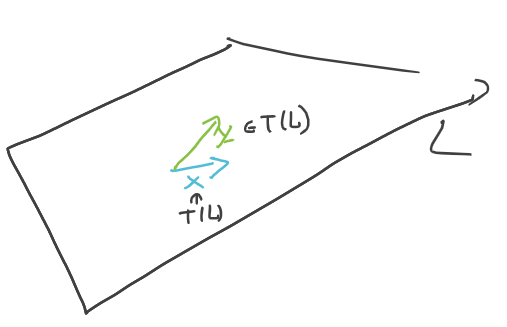
\includegraphics[width=0.5\linewidth]{figures/hyperebene_beispiel_euklidischer_affiner_raum}
    \label{fig:hyperebene_beispiel_euklidischer_affiner_raum}
  \end{figure}
  mit dem aus dem \( \reals^n \) induzierten Standard-Skalarprodukt auf \( T(L)\explain{\text{Untervektorraum}}{\untervektorraum}\reals^n \)
  \begin{equation*}
    \scalarproduct{\cdot}{\cdot}\maps \begin{aligned}[t]
      T(L)\times T(L)&\to \reals\\
      (x,y) &\mapsto \scalarproduct{x}{y}.
    \end{aligned}
  \end{equation*}
\end{beispiel}
\begin{frage*}
  Definition von Abständen / Winkeln in einem euklidischen affinen Raum?
\end{frage*}
\begin{definition}
  Sei \( X \) ein euklidischer affiner Raum. Wir definieren eine Normabbildung
  \begin{equation*}
    \norm*{\cdot}\maps \begin{aligned}[t]
      T(X)&\to \reals_{\geq 0}\\
      t&\mapsto \norm*{t}\definedas \sqrt{\scalarproduct{t}{t}}
    \end{aligned}
  \end{equation*}
  und eine Metrik
  \begin{equation*}
    d\maps \begin{aligned}[t]
      X\times X&\to \reals_{\geq 0}\\
      (p,q)\mapsto \distance{p}{q}\definedas \norm*{\vv{pq}}.
    \end{aligned}
  \end{equation*}
  \begin{figure}[H]
    \centering
    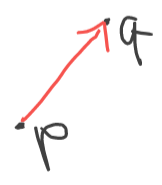
\includegraphics[width=0.2\linewidth]{figures/metrik_auf_affinem_raum_visualisierung}
    \label{fig:metrik_auf_affinem_raum_visualisierung}
  \end{figure}
\end{definition}
\begin{bemerkung*}
  \( \norm*{\cdot} \) ist eine Norm, da \( \scalarproduct{\cdot}{\cdot} \) ein Skalarprodukt ist. Man kann nachrechnen, dass \( d \) tatsächlich eine Metrik auf \( X \) ist, \zb
  \begin{equation*}
    \distance{p}{q}=\norm*{\vv{pq}}=\norm*{-\vv{qp}}=\abs*{-1}\cdot\vv{qp}=\distance{q}{p}.
  \end{equation*}
\end{bemerkung*}
\begin{definition*}
  Sei \( X \) ein euklidischer affiner Raum, \( p,q,q'\in X \) mit \( p\neq q \), \( q' \), \( L=p\vee q \), \( L'=p\vee q' \).
  \begin{figure}[H]
    \centering
    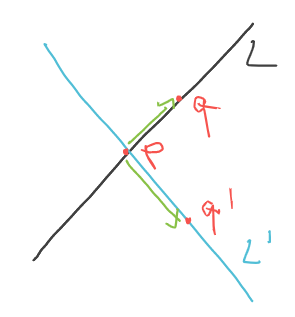
\includegraphics[width=0.5\linewidth]{figures/affiner_winkel_definition}
    \label{fig:affiner_winkel_definition}
  \end{figure}
  Wir definieren den Winkel \( \lineangle{L}{L'} \) zwischen den Geraden \( L,L' \) durch
  \begin{equation*}
    \lineangle{L}{L'}=\arccos \frac{\abs*{\scalarproduct{\vv{pq}}{\vv{pq'}}}}{\norm*{\vv{pq}}\cdot\norm*{\vv{pq'}}}\in \interval{0}{\frac{\pi}{2}}.
  \end{equation*}
  \begin{figure}[H]
    \centering
    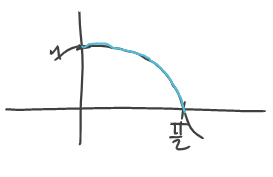
\includegraphics[width=0.3\linewidth]{figures/affiner_winkel_definition_wertebereich}
    \label{fig:affiner_winkel_definition_wertebereich}
  \end{figure}
  \begin{figure}[H]
    \centering
    
\includegraphics[width=0.1\linewidth]{figures/affiner_winkel_definition_wertebereich_beispiel}
    \label{fig:affiner_winkel_definition_wertebereich_beispiel}
  \end{figure}
\end{definition*}
\begin{bemerkung*}
  Die Definition des Winkels \( \lineangle{L}{L'} \) ist unabhängig von der Wahl der Elemente \( q,q' \) (solange \( p\neq q,q' \)).
\end{bemerkung*}